Finden Sie alle L"osungen der Gleichung
\[
z^5+32=0.
\]

\begin{loesung}
\begin{figure}
\centering
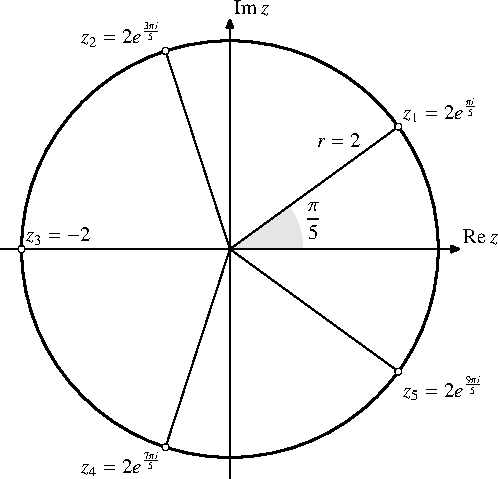
\includegraphics{uebungsaufgaben/exercise-1.pdf}
\caption{L"osungen der Gleichung $z^5+32=0$
\label{skript:15006:loesungen}}
\end{figure}
Wir suchen alle komplexen Zahlen in der Form $z=re^{i\varphi}$, es muss gelten
\begin{align*}
z^5&=r^5e^{5i\varphi}=-32
\\
r&=2\qquad\text{und}\qquad e^{5i\varphi}=-1
\\
\cos 5\varphi+i\sin 5\varphi&=-1
\\
\sin 5\varphi&=0
\\
\cos 5\varphi&=-1
\end{align*}
Die letzte Gleichung besagt, dass $5\varphi$ ein ungerades Vielfaches von
$\pi$ sein muss. Die zweitletzte Gleichung ist schw"acher, sie verlangt
nur, dass $5\varphi$ ein Vielfaches von $\pi$ sein muss, sie ist also
auf jeden Fall erf"ullt, wenn die letzte erf"ullt ist.
\[
5\varphi=(2k+1)\pi
\qquad\Rightarrow\qquad
\varphi=(2k+1)\frac{\pi}5
\]
$\varphi$ muss also ein ungerades Vielfaches von $\frac{\pi}5$ sein:
\[
\varphi\in\biggl\{
e^{i\varphi}\bigg|
\varphi
=
\frac{\pi}{5},
\frac{3\pi}{5},
\frac{5\pi}{5},
\frac{7\pi}{5},
\frac{9\pi}{5}
\biggr\}
\]
In der komplexen Ebene bilden die m"oglichen $\varphi$ ein regelm"assiges
F"unfeck (Abbildung~\ref{skript:15006:loesungen}).
Da das F"unfeck mit Zirkel und Linear konstruierbar ist, kann man
einen Wurzelausdruck f"ur Werte der trigonometrischen Funktionen 
finden, es gilt
\[
\cos\frac{\pi}{5}=\frac{1+\sqrt{5}}4
\qquad
\Rightarrow
\qquad
\sin\frac{\pi}5
=
\sqrt{1-\cos^2\frac{\pi}5}
=
\frac12\sqrt{\frac{5-\sqrt{5}}2}
\]
(siehe auch \cite{skript:pentagon}).
Daraus kann man jetzt auch die Winkelfunktionen f"ur die mehrfachen
Winkel berechnen:
\begin{align*}
\cos\frac{3\pi}5
&=
-\cos\frac{2\pi}5
=
-2\cos^2\frac{\pi}5+1
=
\frac{1-\sqrt{5}}4
\\
\sin\frac{3\pi}5
&=
\sin\frac{2\pi}5
=
2\sin\frac{\pi}5\cos\frac{\pi}5
=
\frac14\sqrt{10+2\sqrt{5}}
\end{align*}
Die "ubrigen Punkte des F"unfecks kann man durch Symmetriebetrachtungen
gewinnen.
Die gesuchten L"osungen sind also
\begin{align*}
z
\in
\biggl\{
&
\frac{1+\sqrt{5}}2+\frac{i}2\sqrt{10-2\sqrt{5}},\quad
\frac{1-\sqrt{5}}2 + \frac{i}2\sqrt{10+2\sqrt{5}},\quad
-2,
\\
&
\frac{1-\sqrt{5}}2 - \frac{i}2\sqrt{10+2\sqrt{5}},\quad
\frac{1+\sqrt{5}}2-\frac{i}2\sqrt{10-2\sqrt{5}}
\biggr\}.
\end{align*}
\end{loesung}

